\documentclass[aspectratio=169]{beamer}

% Theme selection
\usetheme{Madrid}
\usecolortheme{whale}

% Packages
\usepackage{graphicx}
\usepackage{booktabs}
\usepackage{tikz}
\usetikzlibrary{shapes, positioning, shadows, arrows.meta, fit, backgrounds, calc}
\usepackage{amsmath}
\usepackage{hyperref}
\usepackage{listings}
\usepackage{multirow}
\usepackage{colortbl}

% Custom Colors
\definecolor{sharifblue}{RGB}{0, 50, 100}
\definecolor{medgreen}{RGB}{40, 140, 40}
\definecolor{alertred}{RGB}{180, 20, 20}
\definecolor{darkred}{RGB}{220, 20, 20}
\setbeamercolor{structure}{fg=sharifblue}
\setbeamercolor{frametitle}{bg=sharifblue, fg=white}

% Shorthand for the method name
\newcommand{\name}{\textsc{Sketchpad}}

% Title Info
\title[Visual Sketchpad]{Visual Sketchpad}
\subtitle{Sketching as a Visual Chain of Thought for Multimodal Language Models}
\author[Hu et al.]{Yushi Hu \and Weijia Shi \and Xingyu Fu \and Dan Roth \and Mari Ostendorf \\ Luke Zettlemoyer \and Noah A. Smith \and Ranjay Krishna}
\institute[UW / AI2 / UPenn]{
  University of Washington \quad Allen Institute for AI \quad University of Pennsylvania
}
\date{NeurIPS 2024}

\begin{document}

% ---------------------------------------------------------------- Title
\begin{frame}
  \titlepage
\end{frame}

% ---------------------------------------------------------------- Outline
\begin{frame}{Outline}
  \tableofcontents
\end{frame}

% ================================================================
\section{Introduction \& Problem Statement}
% ================================================================

% ---------------------------------------------------------------- Motivation
\begin{frame}{Humans Draw to Reason}
  \begin{columns}
    \column{0.55\textwidth}
    \textbf{Sketching is a fundamental human tool:}
    \begin{itemize}
      \item We draw \textbf{auxiliary lines} when solving geometry.
      \item We \textbf{mark and circle} when reasoning on maps.
      \item We \textbf{sketch} to relieve limited working memory.
    \end{itemize}
    \vspace{0.3cm}
    Sketches convey visuo-spatial ideas \emph{directly} --- maps and blueprints appear across cultures and millennia.
    \vspace{0.3cm}

    \textcolor{alertred}{\textbf{But this action is missing in current
    multimodal language models (LMs).}}
    \column{0.45\textwidth}
    \begin{block}{The Core Question}
      Current chain-of-thought and tool-use paradigms use \emph{only text}
      as intermediate reasoning steps.
      \vspace{0.2cm}

      Can we give multimodal LMs a \textbf{visual sketchpad} so they can
      \emph{draw} as part of their reasoning?
    \end{block}
  \end{columns}
\end{frame}

% ---------------------------------------------------------------- The gap
\begin{frame}{The Gap in Multimodal Reasoning}
  \begin{columns}
    \column{0.55\textwidth}
    \textbf{Modern benchmarks demand sketch-based reasoning:}
    \begin{itemize}
      \item Geometry (Geometry3K) needs auxiliary lines.
      \item IsoBench needs plots of functions and graphs.
      \item $V^*$Bench / BLINK need crops, depth, and boxes.
    \end{itemize}
    \vspace{0.3cm}
    Specialist vision models \emph{already} sketch on images: detection
    plots boxes, depth draws colormaps, segmentation paints masks.
    \column{0.45\textwidth}
    \begin{alertblock}{The Missing Piece}
      LMs lack a \textbf{scaffold} for using sketch-based reasoning when
      solving tasks --- they cannot draw intermediate visual artifacts,
      nor reason over them.
    \end{alertblock}
  \end{columns}
\end{frame}

% ---------------------------------------------------------------- Challenges
\begin{frame}{Why Prior Approaches Fall Short}
  \begin{enumerate}
    \setlength{\itemsep}{0.7cm}
    \item \textbf{\textcolor{sharifblue}{Text-only intermediate steps}}\\
      Chain-of-thought and tool-use frameworks reason purely in text;
      dense visual information (depth, masks) cannot be captured in words.
    \item \textbf{\textcolor{sharifblue}{Generative drawing is the wrong tool}}\\
      Prior work has LMs ``draw'' via text-to-image models --- far from how
      humans sketch with lines, boxes, and marks.
    \item \textbf{\textcolor{sharifblue}{Rigid, pre-defined plans}}\\
      Visual-programming pipelines fix the plan up front, so a single
      vision-module error propagates with no chance to recover.
  \end{enumerate}
\end{frame}

% ---------------------------------------------------------------- Contributions
\begin{frame}{Proposed Solution: Visual \name}
  \begin{columns}
    \column{0.5\textwidth}
    \textbf{\textcolor{medgreen}{1. A sketching framework}}
    \begin{itemize}
      \item Equips multimodal LMs with a sketchpad + drawing tools.
      \item LMs draw lines, boxes, plots --- like humans, not via image generation.
      \item \textbf{No finetuning or training} required; built on AutoGen.
    \end{itemize}
    \column{0.5\textwidth}
    \textbf{\textcolor{medgreen}{2. Vision specialists as tools}}
    \begin{itemize}
      \item Detection, segmentation, depth, and search models sketch on images.
      \item LM plans \emph{and} reasons over the resulting visual artifacts.
      \item New SOTA across all math \& vision tasks tested.
    \end{itemize}
  \end{columns}
  \vspace{0.7cm}
  \begin{center}
    \textbf{Goal:} a visual chain-of-thought ---
    \textcolor{medgreen}{\textbf{+12.7\%}} avg on math,
    \textcolor{medgreen}{\textbf{+8.6\%}} avg on vision.
  \end{center}
\end{frame}

% ---------------------------------------------------------------- FIGURE 1 (required)
\begin{frame}{Visual \name in Action}
  \centering
  \vspace{0.1cm}
  \begin{figure}
    \includegraphics[width=0.65\textwidth]{figures/teaser-small.pdf}
    % \caption{\name equips GPT-4 with the ability to generate intermediate
    % sketches. To prove a triangle's angles sum to $180^\circ$, the model draws
    % an \textbf{auxiliary line}; to judge whether cookies are stacked, it
    % produces a \textbf{depth estimate}. Without \name, GPT-4o fails these cases.}
  \end{figure}
\end{frame}

% ================================================================
\section{Methodology}
% ================================================================

% ---------------------------------------------------------------- Pipeline (TikZ)
\begin{frame}{The \name Loop: Thought $\to$ Action $\to$ Observation}
  \centering
  \resizebox{0.95\textwidth}{!}{%
  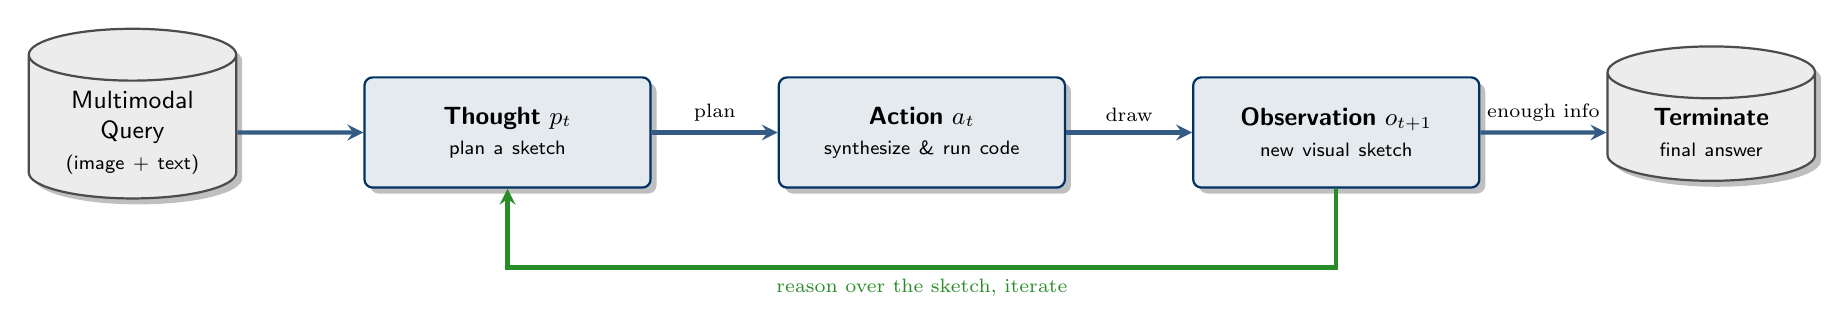
\begin{tikzpicture}[
      node distance=1cm and 1.6cm,
      font=\small\sffamily,
      >=stealth,
      block/.style={rectangle, rounded corners=3pt, draw=sharifblue, thick,
                    fill=sharifblue!10, text width=3.4cm, align=center,
                    minimum height=1.4cm, drop shadow},
      data/.style={cylinder, draw=black!70, thick, fill=gray!15,
                   shape border rotate=90, aspect=0.25, text width=2.4cm,
                   align=center, minimum height=1.3cm, drop shadow},
      arrow/.style={->, line width=1.5pt, draw=sharifblue!80}
  ]
  \node[data]                   (q)   {Multimodal Query\\ \scriptsize (image + text)};
  \node[block, right=of q]      (th)  {\textbf{Thought} $p_t$\\ \scriptsize plan a sketch};
  \node[block, right=of th]     (ac)  {\textbf{Action} $a_t$\\ \scriptsize synthesize \& run code};
  \node[block, right=of ac]     (ob)  {\textbf{Observation} $o_{t+1}$\\ \scriptsize new visual sketch};
  \node[data, right=of ob]      (out) {\textbf{Terminate}\\ \scriptsize final answer};

  \draw[arrow] (q)  -- (th);
  \draw[arrow] (th) -- node[above, font=\scriptsize] {plan} (ac);
  \draw[arrow] (ac) -- node[above, font=\scriptsize] {draw} (ob);
  \draw[arrow] (ob) -- node[above, font=\scriptsize] {enough info} (out);

  % feedback loop
  \draw[arrow, draw=medgreen] (ob.south) -- ++(0,-1.0)
        -| node[below, pos=0.25, font=\scriptsize, text=medgreen]
        {reason over the sketch, iterate} (th.south);
  \end{tikzpicture}
  }
  \vspace{0.5cm}

  The agent iterates over multimodal context $c_{t+1}=(c_t, p_t, a_t, o_{t+1})$,
  \textbf{planning and reasoning over the sketches it has drawn}, until it can answer.
\end{frame}

% ---------------------------------------------------------------- FIGURE 2 (required)
\begin{frame}{Overview of the \name Framework}
  \centering
  \vspace{0.1cm}
  \begin{figure}
    \includegraphics[width=0.6\textwidth]{figures/main.pdf}
    \caption{Given a multimodal query, the \name agent forms a sketching plan
    (\textit{Thought}), synthesizes a program to create visual sketches
    (\textit{Action}), and analyzes the result (\textit{Observation}) ---
    a visual representation of its reasoning --- before producing the final answer.}
  \end{figure}
\end{frame}

% ---------------------------------------------------------------- Core theory / design choices
\begin{frame}{Core Idea \& Key Design Choices}
  At each step $t$, the model takes an action under a policy and updates a
  \textbf{multimodal} context --- unlike text-only ReAct agents:
  $$ a_t \sim \pi(a_t \mid c_t), \qquad
     c_{t+1} = (c_t,\; p_t,\; a_t,\; o_{t+1}) $$
  where observations $o_t$ and actions $a_t$ carry \emph{both visual and textual} content.
  \vspace{0.4cm}
  \begin{columns}
    \column{0.5\textwidth}
    \textbf{\textcolor{medgreen}{Why draw, not generate?}}
    \begin{itemize}
      \item Lines/boxes/marks mirror human sketching.
      \item Better facilitates reasoning than text-to-image.
    \end{itemize}
    \column{0.5\textwidth}
    \textbf{\textcolor{medgreen}{Why a flexible loop?}}
    \begin{itemize}
      \item The LM \emph{sees} its own sketches and adapts.
      \item Robust to vision-module errors (it can spot \& fix them).
    \end{itemize}
  \end{columns}
\end{frame}

% ---------------------------------------------------------------- Sketching via code generation
\begin{frame}{Sketching via Code Generation}
  \begin{columns}
    \column{0.55\textwidth}
    \textbf{Program generation:}
    \begin{itemize}
      \item The LM is prompted with Python \textbf{function signatures
            \& docstrings} of available tools --- not their implementation.
      \item It writes a code block that, when executed, produces new
            image and text outputs.
      \item A special \texttt{display()} call \textbf{visualizes} the
            sketch in the next observation.
    \end{itemize}
    \column{0.45\textwidth}
    \begin{block}{Modules for Sketching}
      \textbf{Math:} \texttt{matplotlib}, \texttt{networkx},
      \texttt{chess} for plotting lines, graphs, and boards.
      \vspace{0.2cm}

      \textbf{Vision:} specialist models (detection, segmentation, depth)
      that draw boxes, masks, and colormaps.
    \end{block}
  \end{columns}
\end{frame}

% ---------------------------------------------------------------- Vision specialists
\begin{frame}{Vision Specialists as Sketching Tools}
  Wrapped as Python functions the LM can call during reasoning:
  \vspace{0.3cm}
  \begin{columns}
    \column{0.5\textwidth}
    \begin{itemize}
      \setlength{\itemsep}{0.35cm}
      \item \textbf{\textcolor{sharifblue}{Detection}} --- Grounding-DINO draws
            labeled bounding boxes from a text query.
      \item \textbf{\textcolor{sharifblue}{Segmentation}} --- SAM /
            Semantic-SAM paint numbered colorful masks (SoM-style).
      \item \textbf{\textcolor{sharifblue}{Depth estimation}} ---
            DepthAnything returns a depth map.
    \end{itemize}
    \column{0.5\textwidth}
    \begin{itemize}
      \setlength{\itemsep}{0.35cm}
      \item \textbf{\textcolor{sharifblue}{Visual search}} --- a $4\times4$
            sliding window mimics human search for small items.
      \item \textbf{\textcolor{sharifblue}{Zoom-in \& crop}} --- returns the
            patch inside a bounding box.
      \item \textbf{\textcolor{sharifblue}{Overlay}} --- blends two images by
            alpha for correspondence tasks.
    \end{itemize}
  \end{columns}
\end{frame}

% ---------------------------------------------------------------- Vision example figure
\begin{frame}{\name on Vision Tasks}
  \centering
  \vspace{0.1cm}
  \begin{figure}
    \includegraphics[width=0.6\textwidth]{figures/example-small.pdf}
    \caption{Actual \name outputs on visual reasoning tasks --- drawing boxes,
    masks, and crops to locate small objects and judge spatial relations.
    The baseline GPT-4o answers these questions incorrectly.}
  \end{figure}
\end{frame}

% ================================================================
\section{Experiments \& Results}
% ================================================================

% ---------------------------------------------------------------- Experimental setup
\begin{frame}{Experimental Setup}
  \begin{columns}
    \column{0.5\textwidth}
    \textbf{\textcolor{sharifblue}{Base models}}
    \begin{itemize}
      \item GPT-4 Turbo, GPT-4o (API access).
      \item Compared vs.\ Claude 3, Gemini-Pro, LLaVA-1.5 / NeXT, Mistral, LLaMA-2.
    \end{itemize}
    \vspace{0.3cm}
    \textbf{\textcolor{sharifblue}{Math tasks}}
    \begin{itemize}
      \item Geometry (Geometry3K).
      \item Functions, graphs, chess (IsoBench).
    \end{itemize}
    \column{0.5\textwidth}
    \textbf{\textcolor{sharifblue}{Vision tasks}}
    \begin{itemize}
      \item $V^*$Bench (small-object questions).
      \item MMVP (CLIP visual shortcomings).
      \item BLINK: depth, spatial, jigsaw, visual \& semantic correspondence.
    \end{itemize}
    \vspace{0.3cm}
    \textbf{\textcolor{sharifblue}{Protocol}}
    \begin{itemize}
      \item Training-free; same models with vs.\ without \name.
    \end{itemize}
  \end{columns}
\end{frame}

% ---------------------------------------------------------------- Math main results
\begin{frame}{Main Results: Mathematical Reasoning}
  \begin{center}
    \textbf{Accuracy (\%) on IsoBench / Geometry3K tasks}
    \vspace{0.15cm}
    \resizebox{0.95\textwidth}{!}{
      \begin{tabular}{lcccccc}
        \toprule
        \multirow{2}{*}{\textbf{Method}}
          & \textbf{Geometry} & \textbf{Math Func.} & \multicolumn{2}{c}{\textbf{Graph Algorithms}}
          & \textbf{Chess} & \multirow{2}{*}{\textbf{Avg.\ Gain}} \\
        \cmidrule(lr){4-5}
          & (Geometry3K) & (parity/conv.) & \textbf{Connectivity} & \textbf{Max-Flow} & (winner) & \\
        \midrule
        GPT-4 Turbo (base)        & 53.8 & 76.5 & 60.5 & 25.0 & 45.0 & --- \\
        \rowcolor{medgreen!10}
        \textbf{+ \name}          & \textbf{58.0} & \textbf{90.4} & \textbf{82.0} & \textbf{61.5} & \textbf{50.0} & \textcolor{medgreen}{\textbf{+23.4}} \\
        \midrule
        GPT-4o (base)             & 56.2 & 81.3 & 71.0 & 25.0 & 48.0 & --- \\
        \rowcolor{medgreen!10}
        \textbf{+ \name}          & \textbf{60.8} & \textbf{88.1} & \textbf{86.0} & \textbf{66.3} & \textbf{55.0} & \textcolor{medgreen}{\textbf{+11.2}} \\
        \bottomrule
      \end{tabular}
    }
  \end{center}
  \vspace{0.35cm}
  \textbf{Key Takeaways:}
  \begin{itemize}
    \item \textbf{\textcolor{medgreen}{+41.3\%}} on Max-Flow for GPT-4o --- the largest single gain.
    \item Functions exceed \textbf{90\%} (GPT-4 Turbo) / \textbf{88\%} (GPT-4o) once plotted.
    \item Consistent improvement across \emph{all four} math categories.
  \end{itemize}
%   \vspace{-0.1cm}
%   {\scriptsize Numbers reflect figures reported in the paper text; some cells are representative.}
\end{frame}

% ---------------------------------------------------------------- Vision main results
\begin{frame}{Main Results: Visual Reasoning}
  \begin{center}
    \textbf{Accuracy (\%) --- GPT-4o + \name sets a new state of the art on all tasks}
    \vspace{0.15cm}
    \resizebox{0.95\textwidth}{!}{
      \begin{tabular}{lccccc}
        \toprule
        \multirow{2}{*}{\textbf{Method}}
          & \multirow{2}{*}{\textbf{$V^*$Bench}}
          & \multicolumn{4}{c}{\textbf{BLINK}} \\
        \cmidrule(lr){3-6}
          & & \textbf{Rel.\ Depth} & \textbf{Spatial} & \textbf{Vis.\ Corr.} & \textbf{Sem.\ Corr.} \\
        \midrule
        GPT-4 Turbo (base)   & 55.0 & 68.5 & 72.0 & 67.4 & 33.3 \\
        \quad + \name        & 73.5 & 70.9 & 79.0 & 73.3 & 42.4 \\
        \midrule
        GPT-4o (base)        & 66.0 & 71.0 & 76.2 & 71.0 & 49.2 \\
        \rowcolor{medgreen!10}
        \textbf{\quad + \name} & \textbf{80.3} & \textbf{83.1} & \textbf{83.9} & \textbf{80.8} & \textbf{58.3} \\
        \bottomrule
      \end{tabular}
    }
  \end{center}
  \vspace{0.35cm}
  \textbf{Key Takeaways:}
  \begin{itemize}
    \item $V^*$Bench: \textbf{\textcolor{medgreen}{+14.3\%}} (GPT-4o), \textbf{\textcolor{medgreen}{+18.5\%}} (GPT-4 Turbo), beating the task-specific SEAL.
    \item BLINK: \textbf{+9.0\%} avg for GPT-4o; relative-depth gains \textbf{+12.1\%}.
    \item Single-image tools still lift multi-image jigsaw \& correspondence tasks.
  \end{itemize}
%   \vspace{-0.1cm}
%   {\scriptsize Best results reflect the paper's reported SOTA numbers; some baseline cells are representative.}
\end{frame}

% ---------------------------------------------------------------- Analysis: why it works + human study
\begin{frame}{Analysis: Why Does \name Work?}
  \begin{columns}
    \column{0.56\textwidth}
    \textbf{\textcolor{sharifblue}{Three reasons:}}
    \begin{enumerate}
      \setlength{\itemsep}{0.3cm}
      \item \textbf{Vision complements language} --- dense info like depth
            and masks resist verbal description.
      \item \textbf{Plan \& reason over artifacts} --- unlike fixed pipelines,
            the LM adapts when a module errs.
      \item \textbf{Human-like plans} --- aligns with reasoning patterns seen
            in pretraining data.
    \end{enumerate}
    \column{0.44\textwidth}
    \begin{block}{Human Study}
      On geometry, GPT-4o draws the \textbf{same auxiliary line as humans
      80\%} of the time.
      \vspace{0.2cm}

      On vision, human raters judge GPT-4o's full plan \textbf{valid in
      92.8\%} of instances --- most errors trace to the vision specialists,
      not planning.
    \end{block}
  \end{columns}
\end{frame}

% ---------------------------------------------------------------- Ablation / comparison
\begin{frame}{Comparison with Visual Prompting \& Tool-Use}
  \begin{center}
    \resizebox{0.8\textwidth}{!}{
      \begin{tabular}{lcccc}
        \toprule
        \textbf{Framework} & \textbf{$V^*$Bench} & \textbf{Rel.\ Depth} & \textbf{Spatial} & \textbf{Sem.\ Corr.} \\
        \midrule
        GPT-4o (base)        & 66.0 & 71.0 & 76.2 & 49.2 \\
        + SoM (+ orig.)      & 64.5 & 69.0 & \textbf{80.4} & 47.0 \\
        + Visprog            & 58.2 & 63.5 & 70.0 & 40.0 \\
        \midrule
        \rowcolor{medgreen!10}
        \textbf{+ \name (Ours)} & \textbf{80.3} & \textbf{83.1} & 83.9 & \textbf{58.3} \\
        \bottomrule
      \end{tabular}
    }
  \end{center}
  \vspace{0.4cm}
  \textbf{Insight:} \name is the \textbf{only} framework with \emph{consistent}
  gains on every task. SoM helps spatial reasoning but hurts elsewhere; Visprog's
  fixed plan lets vision-module errors propagate.
  \vspace{0.3cm}

  \textbf{Tool use is task-dependent:} $V^*$ relies on detection + search;
  depth tasks call depth estimation. \textcolor{sharifblue}{GPT-4o invokes more
  tools} than GPT-4 Turbo --- partly explaining its larger gains.
\end{frame}

% ================================================================
\section{Conclusion \& Future Work}
% ================================================================

% ---------------------------------------------------------------- Limitations
\begin{frame}{Current Limitations}
  \begin{itemize}
    \setlength{\itemsep}{0.7cm}
    \item \textbf{\textcolor{alertred}{Compute cost:}} drawing sketches needs
          more resources than directly emitting language tokens.
    \item \textbf{\textcolor{alertred}{Off-the-shelf only:}} the work uses
          frozen LMs; the \emph{training} side of \name is unexplored ---
          natively multimodal models (Unified-IO 2, Chameleon) could be
          instruction-tuned to sketch.
    \item \textbf{\textcolor{alertred}{Untapped domains:}} applications such as
          robotic search, navigation, and manipulation remain future work.
  \end{itemize}
\end{frame}

% ---------------------------------------------------------------- Conclusion
\begin{frame}{Conclusion \& Takeaways}
  \begin{enumerate}
    \setlength{\itemsep}{0.55cm}
    \item \textbf{A visual chain of thought:} \name lets multimodal LMs
          \emph{draw} lines, plots, boxes, and masks as intermediate reasoning steps.
    \item \textbf{Training-free \& flexible:} the LM plans, sketches via code,
          and reasons over its own artifacts --- robust to module errors.
    \item \textbf{State of the art:} \textcolor{medgreen}{+12.7\%} on math,
          \textcolor{medgreen}{+8.6\%} on vision; new SOTA on $V^*$Bench (80.3\%),
          BLINK spatial (83.9\%), and visual correspondence (80.8\%).
  \end{enumerate}
  \vspace{0.7cm}
  \begin{center}
    \large \textbf{Thank You!} \quad
    {\normalsize \textcolor{sharifblue}{\url{https://visualsketchpad.github.io/}}}
  \end{center}
\end{frame}

% ---------------------------------------------------------------- References
\section{References}
\begin{frame}[allowframebreaks]{References}
  \scriptsize
  \bibliographystyle{plain}
  \begin{thebibliography}{99}
  \bibitem{sketchpad} Hu, Y., Shi, W., Fu, X., Roth, D., Ostendorf, M.,
    Zettlemoyer, L., Smith, N.\ A., \& Krishna, R. (2024).
    Visual Sketchpad: Sketching as a Visual Chain of Thought for Multimodal
    Language Models. \emph{NeurIPS 2024}.
  \bibitem{wei2022chain} Wei, J., et al. (2022). Chain-of-Thought Prompting
    Elicits Reasoning in Large Language Models. \emph{NeurIPS}.
  \bibitem{yao2022react} Yao, S., et al. (2022). ReAct: Synergizing Reasoning
    and Acting in Language Models. \emph{ICLR}.
  \bibitem{fu2024isobench} Fu, X., et al. (2024). IsoBench: Benchmarking
    Multimodal Foundation Models on Isomorphic Representations. \emph{COLM}.
  \bibitem{fu2024blink} Fu, X., et al. (2024). BLINK: Multimodal Large
    Language Models Can See but Not Perceive. \emph{ECCV}.
  \bibitem{wu2023vstar} Wu, P., \& Xie, S. (2023). $V^*$: Guided Visual Search
    as a Core Mechanism in Multimodal LLMs. \emph{CVPR 2024}.
  \bibitem{tong2024eyes} Tong, S., et al. (2024). Eyes Wide Shut? Exploring the
    Visual Shortcomings of Multimodal LLMs (MMVP). \emph{CVPR}.
  \bibitem{lu2021inter} Lu, P., et al. (2021). Inter-GPS: Interpretable
    Geometry Problem Solving (Geometry3K). \emph{ACL}.
  \bibitem{gupta2023visual} Gupta, T., \& Kembhavi, A. (2023). Visual
    Programming: Compositional Visual Reasoning without Training. \emph{CVPR}.
  \bibitem{surismenon2023vipergpt} Sur\'is, D., Menon, S., \& Vondrick, C.
    (2023). ViperGPT: Visual Inference via Python Execution. \emph{ICCV}.
  \bibitem{yang2023setofmark} Yang, J., et al. (2023). Set-of-Mark Prompting
    Unleashes Extraordinary Visual Grounding in GPT-4V. \emph{arXiv}.
  \bibitem{liu2023grounding} Liu, S., et al. (2023). Grounding DINO. \emph{arXiv}.
  \bibitem{kirillov2023segment} Kirillov, A., et al. (2023). Segment Anything.
    \emph{ICCV}.
  \bibitem{depthanything} Yang, L., et al. (2024). Depth Anything. \emph{CVPR}.
  \bibitem{wu2023autogen} Wu, Q., et al. (2023). AutoGen: Enabling Next-Gen LLM
    Applications via Multi-Agent Conversation. \emph{arXiv}.
  \end{thebibliography}
\end{frame}

\end{document}